\section{Para saber más}

\begin{frame}[t]{Sitios para saber más}
\begin{itemize}
  \item Fundación ISO C++: \textgood{\url{https://isocpp.org/}}
  
  \vfill
  \item C++ Reference: \textgood{\url{https://en.cppreference.com/}}

  \vfill
  \item Compiler Explorer: \textgood{\url{https://godbolt.org/}}
\end{itemize}
\end{frame}

\begin{frame}[t]{Libros}
\begin{columns}
\column{.2\textwidth}
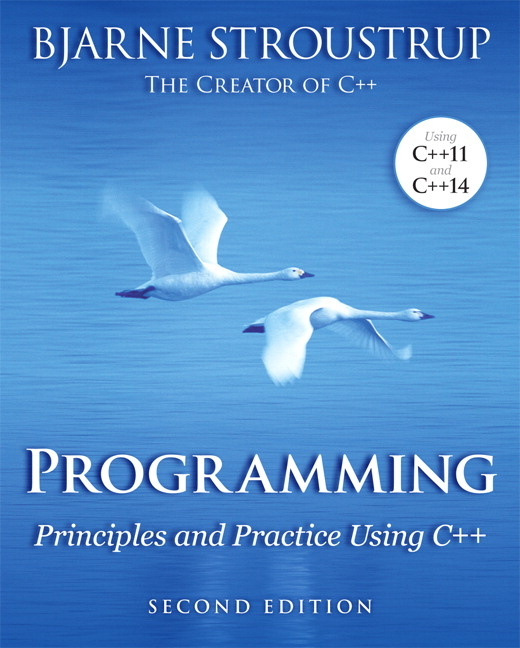
\includegraphics[height=.3\textheight]{img/ppp-2e.jpg}
\column{.8\textwidth}
\begin{itemize}
\item Programming Principles and Practice using C++.\\
      Bjarne Stroustrup.\\
      Segunda edición (tercera inminente).
\end{itemize}
\end{columns}

\vfill

\begin{columns}
\column{.2\textwidth}
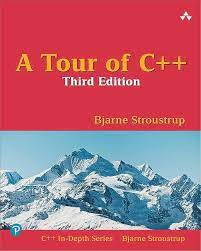
\includegraphics[height=.3\textheight]{img/tour-cpp.jpg}
\column{.8\textwidth}
\begin{itemize}
\item A Tour of C++.\\
      Bjarne Stroustrup.\\
      Tercera edición.
\end{itemize}
\end{columns}
\end{frame}

\begin{frame}[t]{Canales}
\begin{itemize}
  \item CppCon: \url{https://www.youtube.com/@CppCon}

  \vfill
  \item ACCU Conference: \url{https://www.youtube.com/@ACCUConf}

  \vfill
  \item Meeting C++: \url{https://www.youtube.com/@MeetingCPP}

  \vfill
  \item C++ Now: \url{https://www.youtube.com/@BoostCon}

  \vfill
  \item \textgood{using std::cpp}: \url{https://www.youtube.com/@usingstdcpp7242}
\end{itemize}
\end{frame}
